\vspace{-5pt}

\section{Motivation}
\label{sec:motivation}
Through a set of controlled experiments (here and in \S\ref{sec:additional_results_section_3}), we validate three hypotheses that underpin the design of \Feather: (i) prefix homogeneity, the extent to which \textit{all} requests in a batch share a common prefix, has a strong impact on the decode throughput because it increases the locality of KV cache accesses. Importantly, these gains can be achieved \textit{without any modifications to existing attention kernels}. (ii) There is a trade-off between batch size and prefix homogeneity, where moderately sized homogeneous batches \textit{can} outperform large heterogeneous batches; and (iii) existing prefix detection approaches incur substantial CPU overhead. 

\vspace{-5pt}

\subsubsection*{Experimental Setup} 
All experiments use the Llama 3 8B \cite{llama3modelcard} model and are run on an RTX 6000 Ada GPU~\cite{nvidia_rtx6000_datasheet} with 48 GB of GDDR6 memory and a 96 MB L2 cache. We use the vLLM \cite{kwon2023efficient} inference engine with a default maximum batch size of 500 unless stated otherwise. We first focus on decode throughput, measured in output tokens per second. To isolate decode behavior, we perform a warm-up run so that the prefix KV caches are resident in GPU memory. This ensures that per-token compute remains constant within an experiment and differences arise primarily from memory accesses and batching. We also report end-to-end throughput, which includes the time taken to prefill the queries. For this model, a 10k-token request generates 1.2 GB of KV cache data across all layers. Within each layer, vLLM uses its paged memory management system and allocates the KV cache in blocks of 16 tokens contiguously in GPU memory, which is sufficient for locality benefits to kick in. We sample requests from the L-Eval~\cite{an2023leval} dataset and prune the size of each request as required by the experiment. We use the FlashAttention~\cite{dao2022flashattentionfastmemoryefficientexact} backend throughout all the experiments.

\vspace{-8pt}

\subsection{Significance of Prefix Homogeneity}
\label{subsec:significance_of_prefix_homogeneity}
We start by observing the impact of prefix homogeneity on decode phase throughput. When \textit{all} requests in a batch share a common prefix, their attention operations traverse the same KV cache regions concurrently. This yields two beneficial effects: (i) spatial locality: Sequential access to contiguous KV tensors enables the hardware prefetcher to fetch upcoming cache lines from DRAM into L2; (ii) temporal locality: Cache lines fetched for one request are reused by neighboring requests before eviction. Together, these effects increase L2 hit rates and DRAM utilization, improving throughput. In contrast, heterogeneous prefixes interleave KV accesses across disjoint regions, disrupting locality and reducing effective memory bandwidth. We will now present experiments that validate these claims.

\textbf{Experiment 1:} We consider two prefixes, $A$ and $B$, each 10K tokens long. We form a batch of $500$ requests, each using the prefix $A$ or $B$, followed by a unique suffix of length $20$ tokens (\S\ref{subsec:two_large_prefixes_heterogeneity}). Each request generates 50 decode tokens. Let $f \in [0,1]$ denote the fraction of requests using prefix $A$. When $f$ is 0 or 1, the batch is homogeneous; otherwise, two prefix groups coexist. We perform a warm-up run so that KV caches for both prefixes are resident in GPU memory.

Figure~\ref{fig:two_fam_tp} shows decode throughput as a function of $f$. We see that the throughput is highest for fully homogeneous batches. However, even a single request from the other prefix group (e.g., $f = 0.002$) causes throughput to drop by nearly $2\times$. This demonstrates that decode throughput is highly sensitive to even minimal prefix heterogeneity. To understand this effect, we capture DRAM bandwidth utilization using DCGMI~\cite{nvidia_dcgm_2026}. We first plot the mean bandwidth utilization for each $f$, and then we sum the utilization over the entire experiment duration (i.e., compute the area under the memory bandwidth curve) to approximate total memory accesses. As shown in Figure~\ref{fig:two_fam_mean_dram}, homogeneous batches achieve over 40\% higher bandwidth utilization than mixed-prefix batches due to greater spatial locality, enabling more efficient hardware-level prefetching into the GPU cache. Furthermore, greater temporal locality in prefix-homogeneous batches reduces the total data fetched from DRAM. Because most SMs process queries from the dominant prefix even when $f = 0.002$, we attribute the performance gains primarily to improved L2 cache reuse rather than increased L1 cache locality. 

\textbf{Takeaway 1:} \textit{Decode throughput is maximized when \textit{all} requests share a prefix; even a single divergent prefix disrupts locality and sharply reduces effective bandwidth.}

\begin{figure}[t]
\captionsetup[subfigure]{labelformat=simple}
    \renewcommand\thesubfigure{(\alph{subfigure})}
\centering
\begin{subfigure}{0.45\columnwidth}
    \centering
    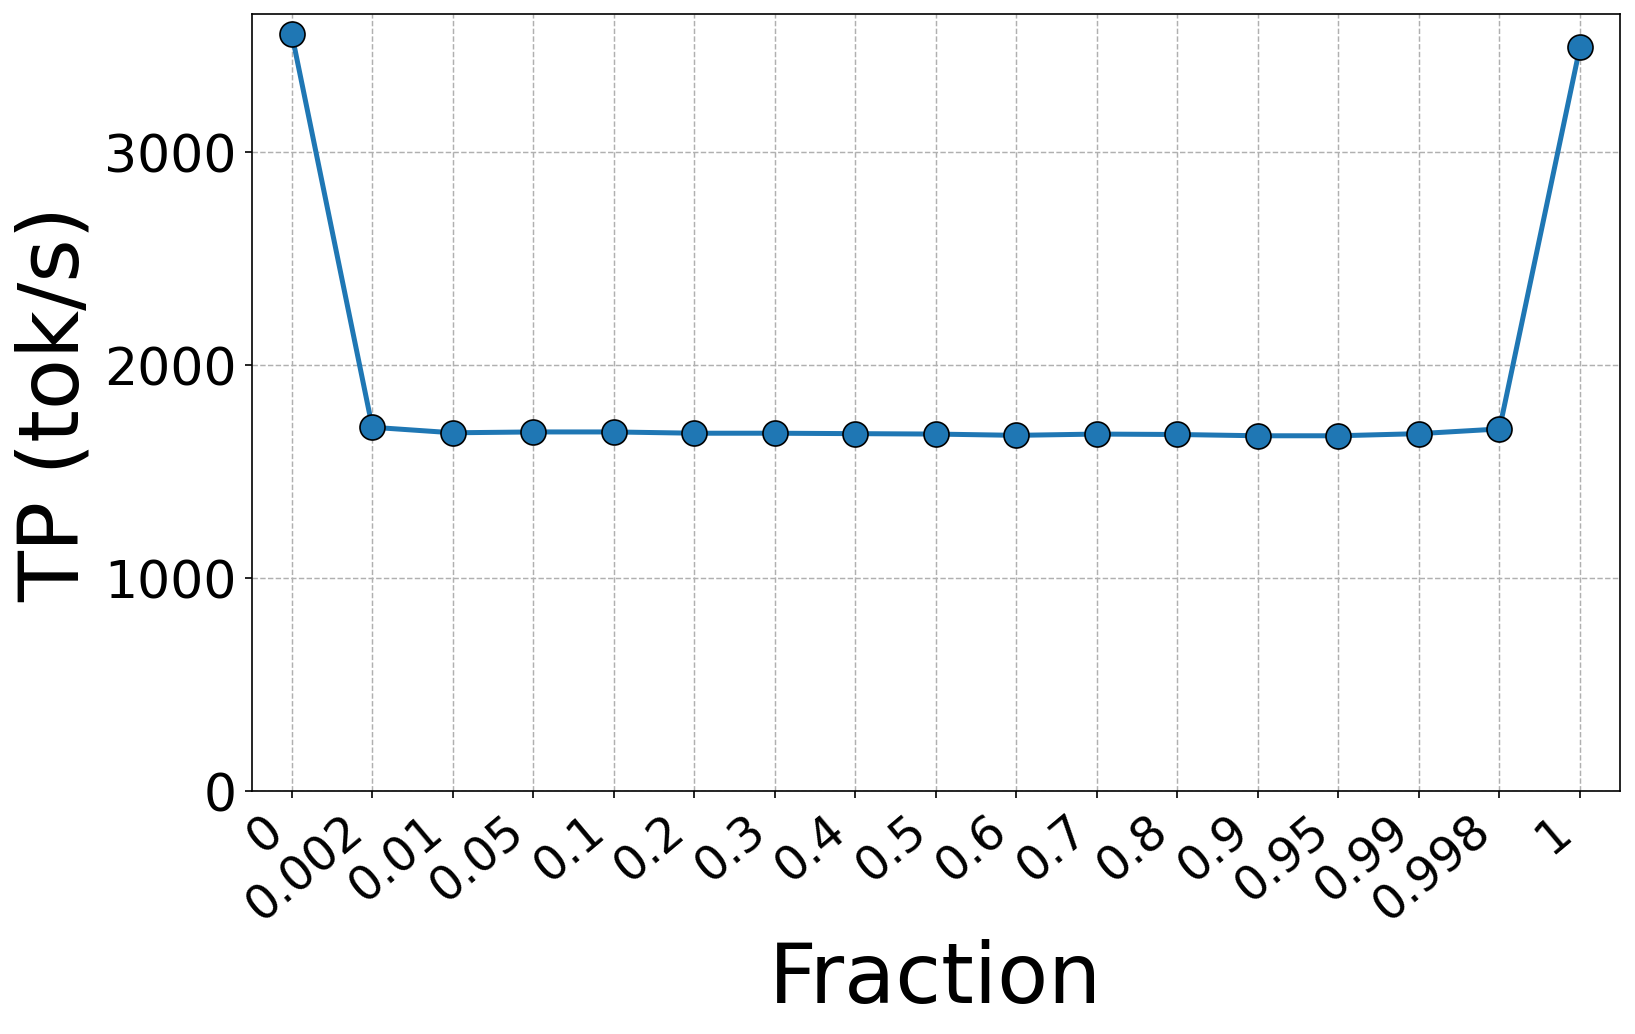
\includegraphics[width=\linewidth]{results/two_family_plots/throughput_vs_fraction.png}
    \caption{Throughput}
    \label{fig:two_fam_tp}
\end{subfigure}
\hfill
\begin{subfigure}{0.45\columnwidth}
    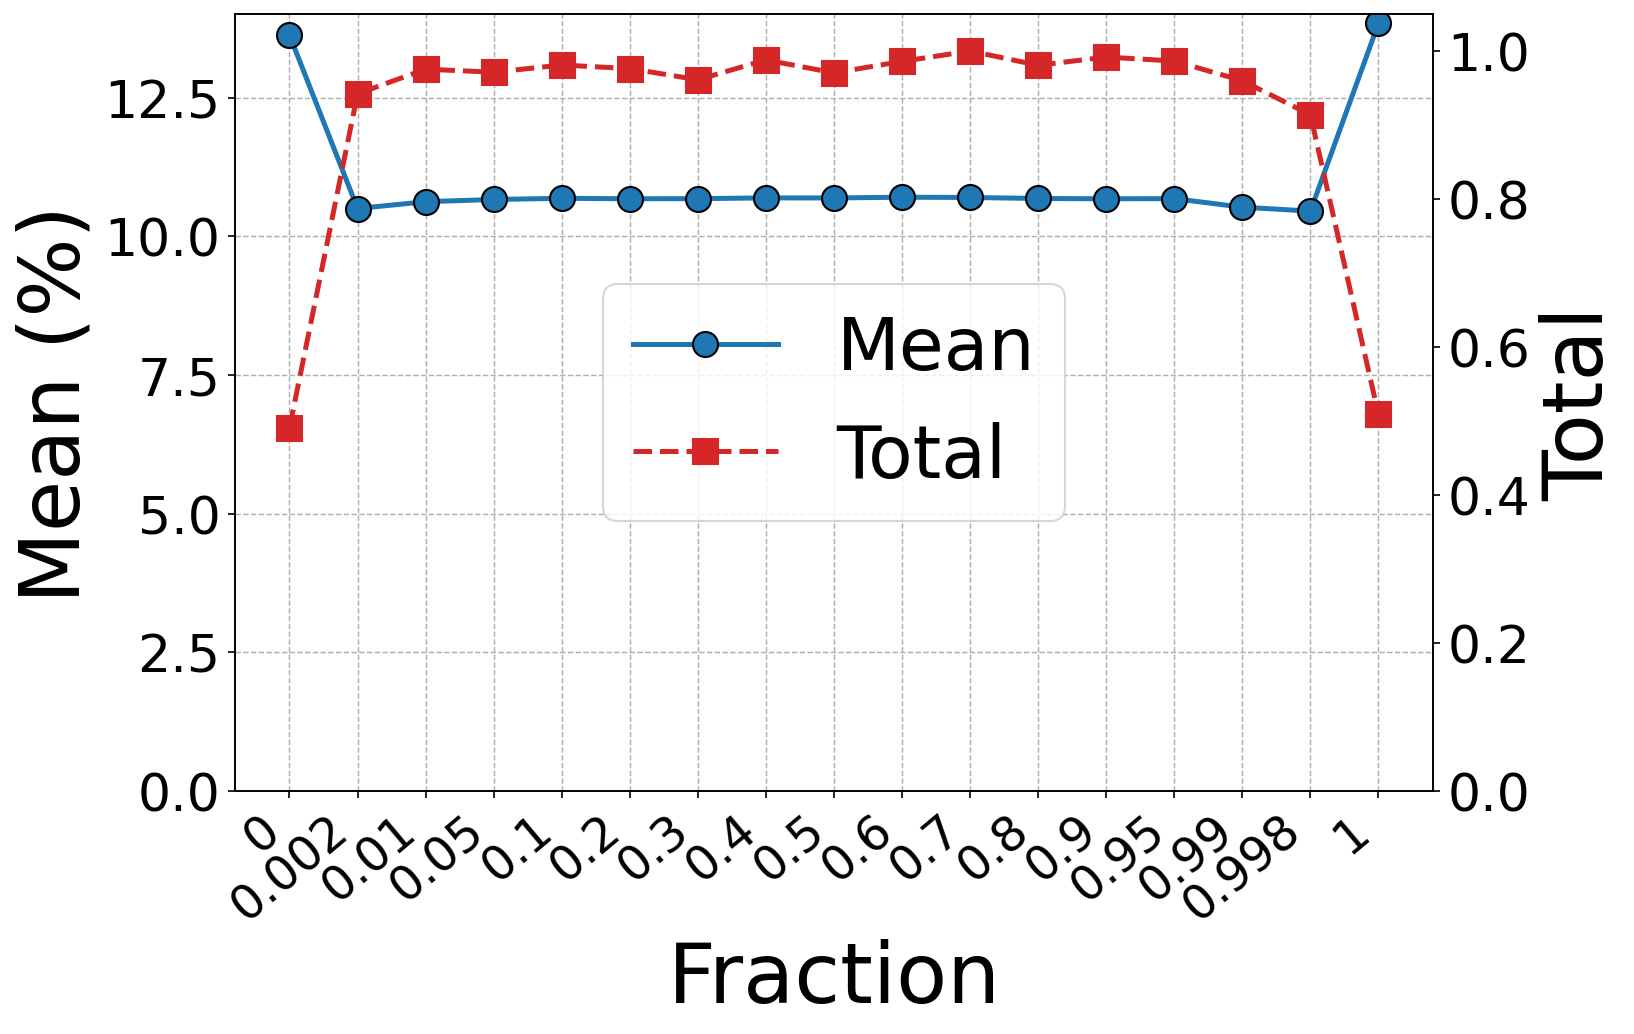
\includegraphics[width=\linewidth]{results/two_family_plots/dcgmi_mean_vs_sum_dual.png}
\caption{Bandwidth Utilization}
\label{fig:two_fam_mean_dram}
\end{subfigure}
\caption{Prefix Homogeneity - Two Prefix Groups}
\label{fig:two_fam_fraction}
\vspace{-20pt}
\end{figure}

\textbf{Experiment 2:} Next, we evaluate the impact of the shared prefix length on performance. For this, we construct a batch of 100 requests, each 2K tokens long and sharing a common prefix of length $2K \times f$ tokens, where $f \in [0, 1]$. The remaining $2K \times (1-f)$ tokens are unique across requests (\S\ref{subsec:fractional_sharing}). The KV caches fit into GPU memory for all values of $f$. Figure~\ref{fig:frac_share_tp} shows that throughput increases smoothly with $f$. It is lowest at $f = 0$ and improves steadily as sharing increases, reaching over 60\% higher throughput at $f = 1$. As $f$ grows, a larger portion of the KV cache is shared across requests; since decode repeatedly traverses the KV cache, greater spatial and temporal locality improve throughput.

\begin{figure}[t]
\centering
\begin{minipage}{0.40\columnwidth}
    \centering
    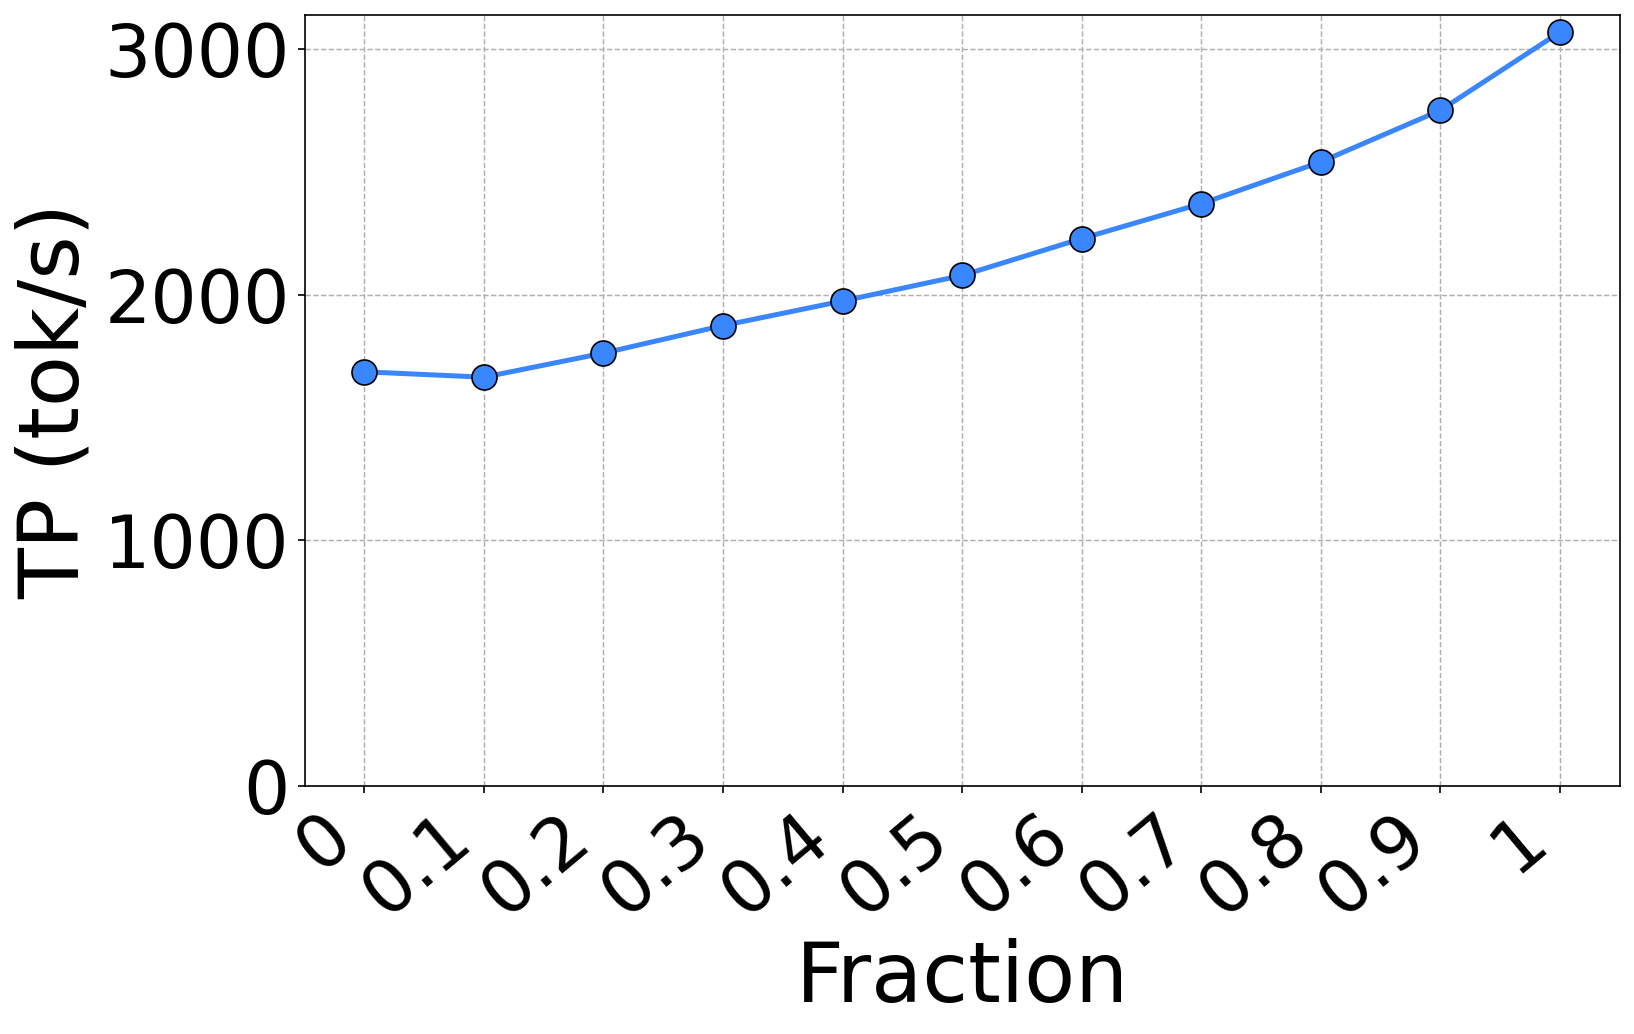
\includegraphics[width=\columnwidth]{results/fractional_sharing_plots/throughput_vs_fraction.png}
    \caption{Fraction of Prefix Shared}
    \label{fig:frac_share_tp}
\end{minipage}
\hfill
\begin{minipage}{0.59\columnwidth}
    \centering
    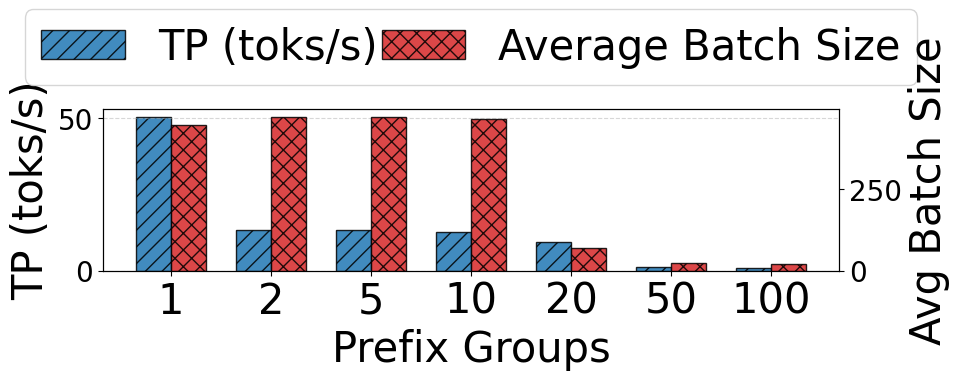
\includegraphics[width=\columnwidth]{results/hbm_evictions_fcfs_throughput_vs_batchsize_dual_axis.png}
    \captionof{figure}{Number of Prefix Groups}
    \label{fig:hbm_evic_tp_bs}
\end{minipage}
\vspace{-20pt}
\end{figure}

\textbf{Takeaway 2:} \textit{In prefix-homogeneous batches, decode throughput increases smoothly with the length of the shared prefix.}

\textbf{Experiment 3:} Next, we evaluate the effect of the number of prefix groups on performance using an experiment with $N$ shared prefixes $P_1, P_2, \dots, P_N$, each of length $10K$ tokens and having same number of requests. Figure~\ref{fig:hbm_evic_tp_bs} shows throughput and average batch size as $N$ increases. As observed earlier, throughput drops from $N = 1$ to $N = 2$ due to reduced temporal and spatial locality arising from prefix heterogeneity. However, from $N = 2$ to $N = 20$, throughput remains stable, indicating that additional heterogeneity has a limited impact once locality is disrupted. Finally, throughput drops sharply from $N = 20$ to $N = 100$, as GPU memory can no longer hold KV caches for all active prefixes. The impact is also visible through the reduced average batch size for $N = 50$ and $N = 100$. Prior work~\cite{zheng2025batchllmoptimizinglargebatched,zheng2024sglangefficientexecutionstructured} mitigates the throughput drop from $N = 20$ to $N = 50$ due to KV cache evictions by maximizing prefix reuse and minimizing memory footprint using depth-first traversal of radix trees. However, to the best of our knowledge, no prior work has observed the drop in performance from $N = 1$ to $N = 2$ prefix groups.

\textbf{Takeaway 3:} \textit{While prefix heterogeneity causes a drop in throughput, the amount of heterogeneity has a marginal impact on the loss of locality. However, very high heterogeneity leads to minimal KV reuse and higher GPU memory evictions.}

\begin{figure*}[t]
\centering
\begin{minipage}{0.30\textwidth}
\centering
    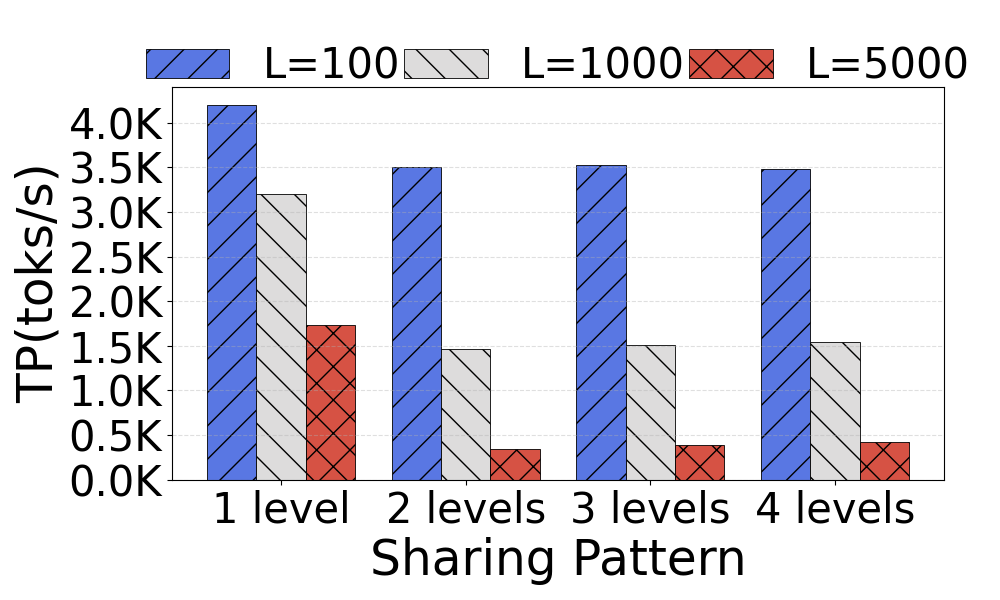
\includegraphics[width=\columnwidth]{results/tp_different_modes_sharing_at_top.png}
    \caption{Radix Tree Sharing Patterns}
    \label{fig:tp_vs_l_1_9_11}
\end{minipage}
\hfill
\begin{minipage}{0.34\textwidth}
    \centering
    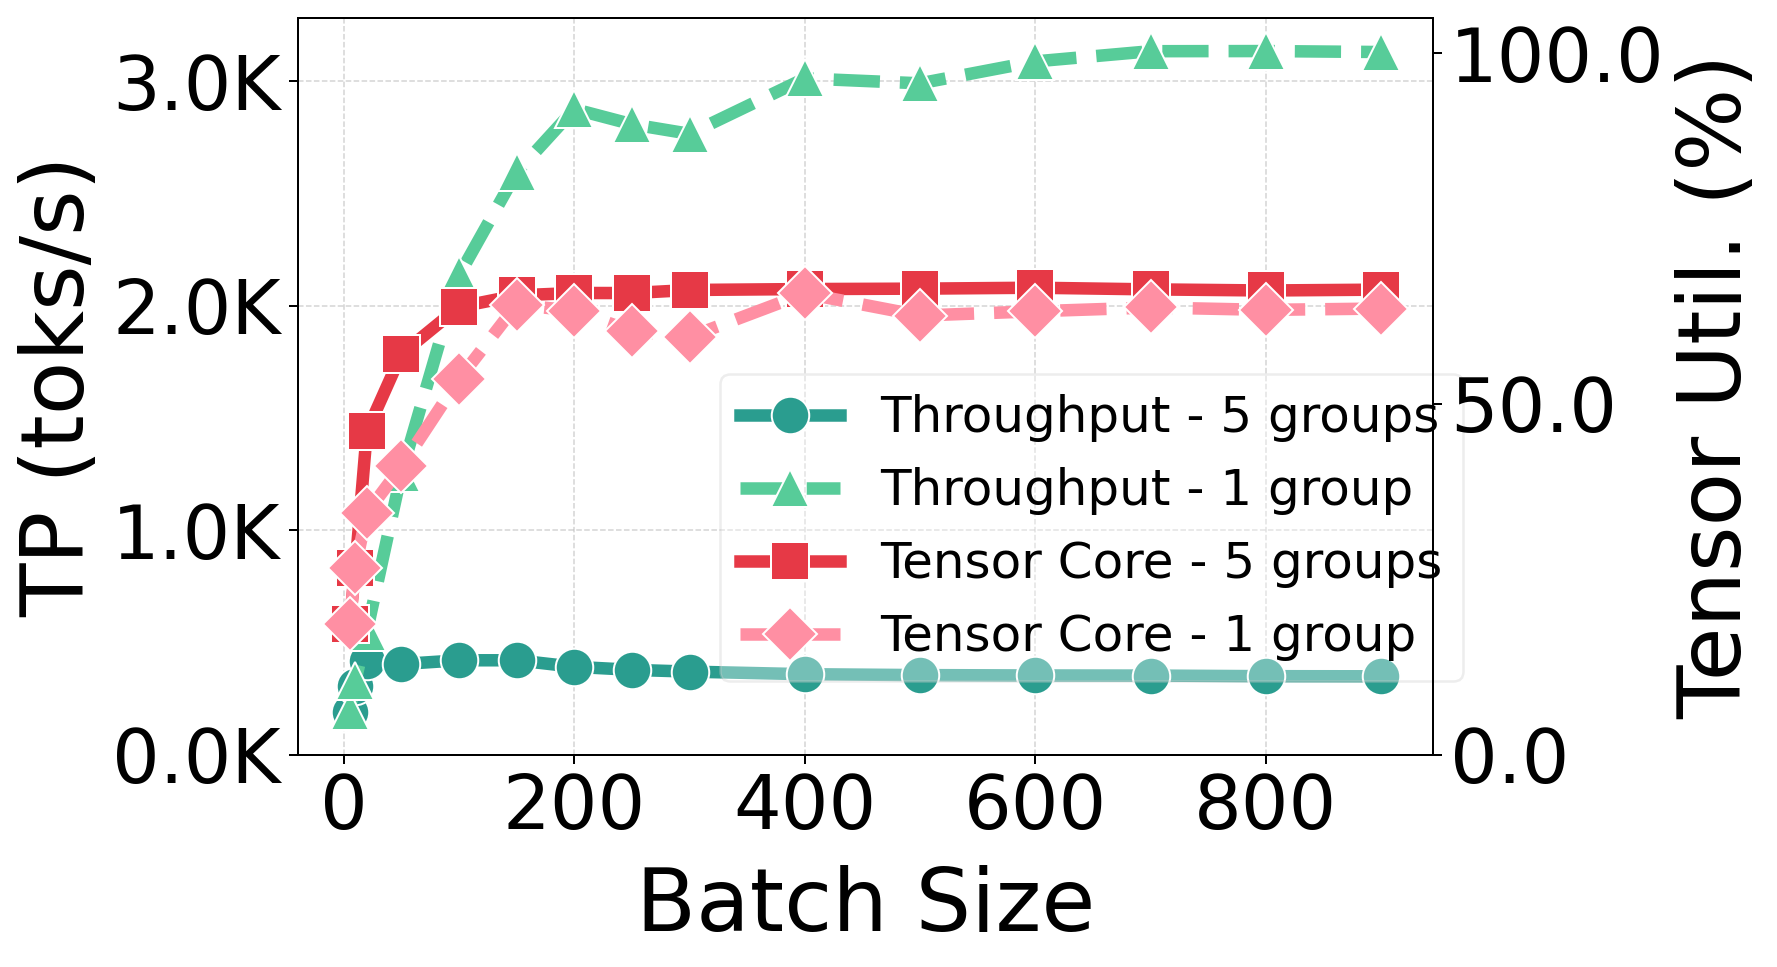
\includegraphics[width=\columnwidth]{results/merged_batch_size_plots/plot1_throughput_tensor_merged.png}
    \captionof{figure}{Throughput vs. Batch Size}
    \label{fig:batch_size_tp_motivation}
\end{minipage}
\hfill
\begin{minipage}{0.34\textwidth}
    \centering
    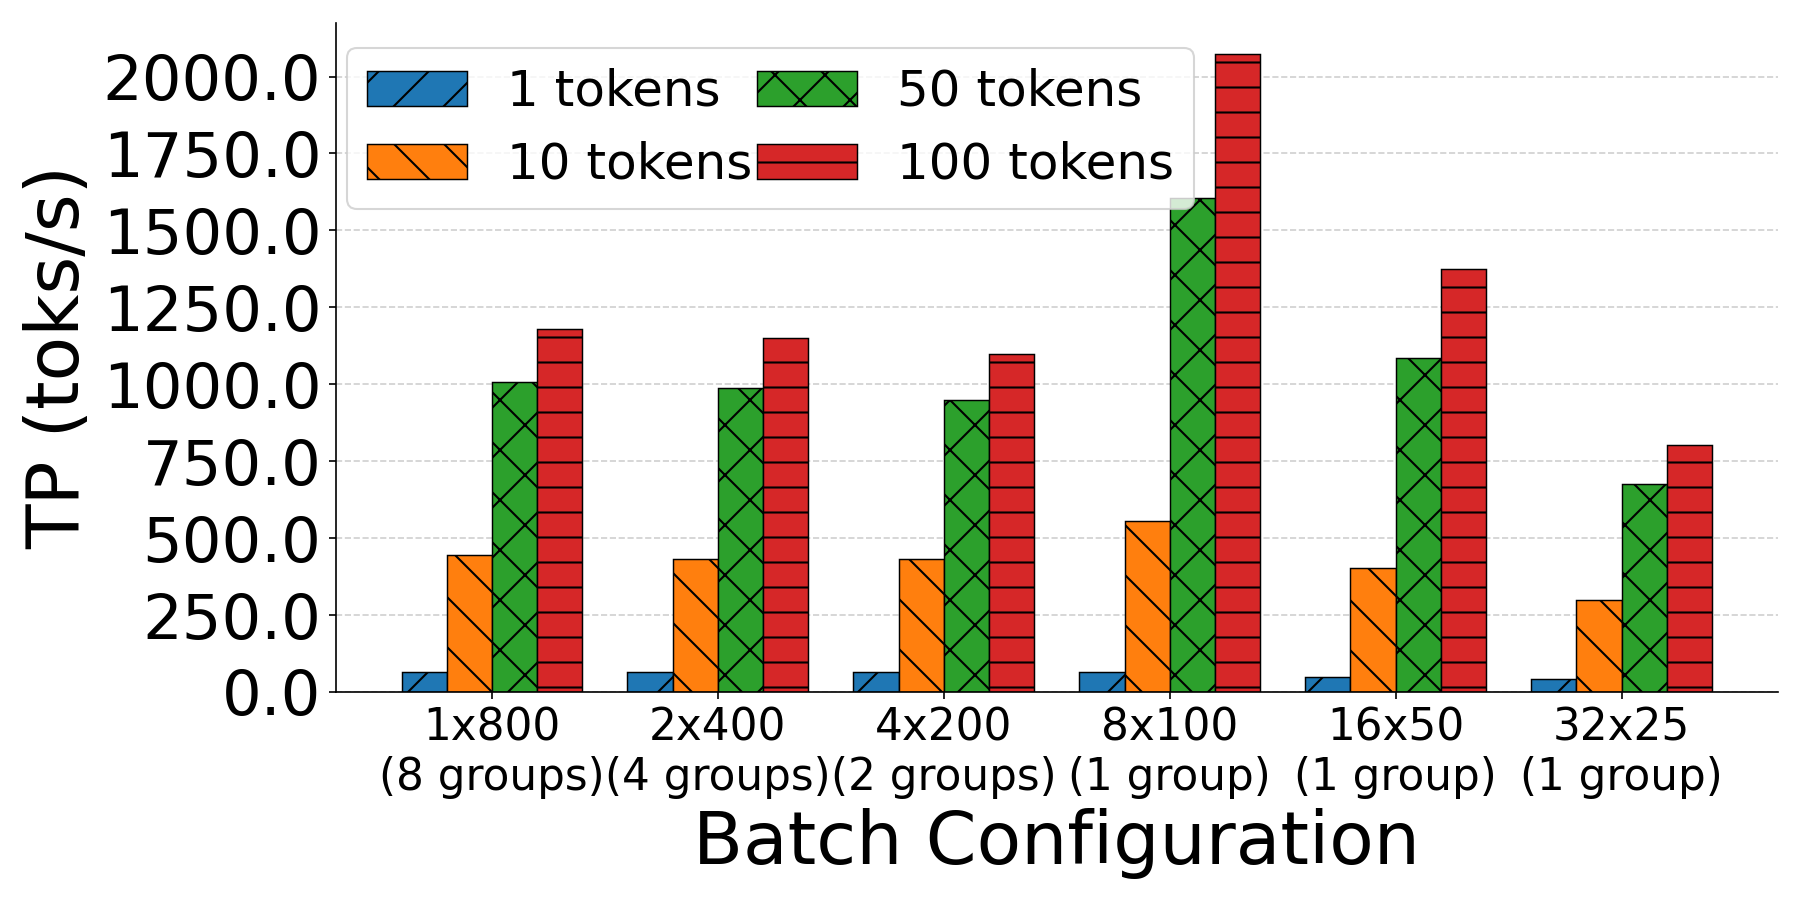
\includegraphics[width=\columnwidth]{results/prefill_decode_homo_hetero_grouped_throughput.png}
    \captionof{figure}{Batch Size vs. Homogeneity}
    \label{fig:prefill_decode_tp_batch_config_decode}
\end{minipage}
\vspace{-15pt}
\end{figure*}

\textbf{Experiment 4:} Until now, all the experiments have considered requests that have a single level of prefix sharing. We now ask the question: what is the impact of more complicated sharing patterns on performance? For this, we construct radix trees with 1 to 4 levels of shared prefixes (\S\ref{subsec:radix_tree_sharing_patterns}). There are two branches in each level, and requests are equally distributed across the leaves. The sequence length per request is fixed at $4L$, and Figure~\ref{fig:tp_vs_l_1_9_11} shows the decode throughput for three values of $L$. As expected, a single level of radix tree has the highest performance because of maximum locality. Interestingly, radix trees with 2, 3, and 4 levels exhibit similar throughput across different values of $L$, despite differing branching structures. Why so? During the initial segment of length $L$, all configurations access the same KV region. However, once branching occurs, the batch becomes heterogeneous, locality degrades, and the marginal cost of additional prefix groups is small, as established earlier in Figure~\ref{fig:hbm_evic_tp_bs}.

\textbf{Takeaway 4:} \textit{Performance is driven mainly by the length of the top-level prefix shared by all requests, while the number of radix-tree levels and branches has a negligible impact.}



\vspace{-10pt}

\subsection{Batch Size vs Prefix Homogeneity}
\label{subsec:batch_size_vs_prefix_homogeneity}
So far, we have established that prefix homogeneity has a significant impact on performance. But when the workload does not have enough requests from a prefix group and prefix-homogeneous batches are too small, the compute will remain under-utilized, leading to a loss in throughput. Therefore, there exists a trade-off between batch size and prefix homogeneity. We now explore this trade-off.

\textbf{Experiment 5:} We study decode throughput vs. batch size using two workloads: (i) heterogeneous, with requests spread across 5 distinct 10K-token prefixes, and (ii) homogeneous, with all requests sharing one such prefix. Figure~\ref{fig:batch_size_tp_motivation} shows throughput and tensor core utilization as a function of batch size for both workloads. We see that throughput plateaus at a point before the maximum batch size, and the saturation throughput is higher in the homogeneous case due to greater locality. Further, the batch size at which throughput saturates is higher for the homogeneous workload because requests can access the same KV cache without using additional memory bandwidth. Interestingly, the compute utilization is almost exactly the same across both workloads.

\textbf{Takeaway 5:} \textit{Decode is memory bandwidth bound and increasing batch size beyond a point does not necessarily improve throughput. However, the point at which diminishing returns begin depends on prefix homogeneity (and hardware config).}

\textbf{Experiment 6:} Given that batch size has a diminishing impact on performance, we ask if moderately small homogeneous batches can outperform larger heterogeneous ones. To answer this, we use eight prefix groups with 100 requests each (800 total, each 10K tokens) and evaluate the following batching strategies: (i) 1$\times$800 (8 prefix groups/batch); (ii) 2$\times$400 (4 prefix groups/batch); (iii) 4$\times$200 (2 prefix groups/ batch); (iv) 8$\times$100 (homogeneous); (v) 16$\times$50 (homogeneous); and (vi) 32$\times$25 (homogeneous). We vary the decode length from 1 to 100 tokens and measure the end-to-end throughput, including both the prefill and decode phases for all batches. Figure~\ref{fig:prefill_decode_tp_batch_config_decode} shows this throughput across the different batching strategies. For small decode lengths, throughput is dominated by prefill, and large heterogeneous batches perform the best due to higher tensor core utilization; splitting 1$\times$800 into smaller batches slightly reduces throughput due to lower compute efficiency, as locality benefits are not yet dominant. As decode length increases, performance trends reverse: multiple decode iterations repeatedly sweep the KV cache and reap greater benefits due to locality. Therefore, at longer decode lengths, fully homogeneous batches (8$\times$100) significantly improve throughput despite smaller batch sizes. Notably, even 16$\times$50 continues to outperform 1$\times$800 at large decode lengths, showing that locality gains can outweigh reduced tensor core utilization. Only when batches become too small (32$\times$25) does throughput decline again, as reduced arithmetic intensity and occupancy dominate.
 
\textbf{Takeaway 6:} \textit{Moderately small prefix-homogeneous batches can achieve higher throughput than larger heterogeneous ones. Gains increase with longer decode lengths as repeated KV sweeps amplify locality; however, excessively small batches underutilize compute and degrade performance.}

\begin{table}[t]
\centering
\small
\resizebox{\columnwidth}{!}{\begin{tabular}{lcccc}
\toprule
\textbf{Policy} & \textbf{Exec (s)} & \textbf{Batch Time (s, \%)} & \textbf{Throughput (toks/s)} \\
\midrule
vLLM FCFS & 229.36 & 3e-6 (0.00\%) & 436.25  \\
SGLANG DFS-W & 177.78 & 92.15 (51.8\%) & 562.61 \\
SGLANG LPM & 149.27 & 46.62 (31.2\%) & 669.92  \\
PAT (vLLM Block Table) & 316.45 & 91.72 (29.0\%) & 316.63  \\
vLLM RadixTree & 139.33 & 62.95 (45.2\%) & 717.35  \\
vLLM User IDs & 105.43 & 0.03 (0.03\%) & 948.54 \\
\bottomrule
\end{tabular}}
\caption{Overhead of Dynamic Prefix Detection}
\label{tab:cost_schedulers}
\vspace{-20pt}
\end{table}

\vspace{-8pt}

\subsection{Overhead of Dynamic Prefix Detection}
\label{subsec:overhead_dynamic_prefix_detection}
Next, we study how state-of-the-art inference engines identify prefix sharing and the costs involved. Systems such as SGLang \cite{zheng2024sglangefficientexecutionstructured} and BatchLLM \cite{zheng2025batchllmoptimizinglargebatched} do not explicitly form prefix-homogeneous batches, but use radix trees to detect sharing, and schedule requests to minimize KV recomputation. 

\textbf{Experiment 7:} We construct a workload of 2K requests, each with a 10K-token prefix, and compare scheduling CPU time to total execution time. SGLang proposes two prefix-aware policies that use its radix tree: \textit{Longest Prefix Match}, which prioritizes requests with the longest matching cached prefixes, and \textit{DFS-Weight}, which performs a depth-first traversal and prioritizes branches with more active requests. vLLM uses a much simpler hash-based block table, which is used for grouping requests in the prefix-aware attention kernel implementation of PAT~\cite{yi2026pat}. We compare the overheads of this block table along with our own radix-tree-based scheduler implemented on top of vLLM. We also compare against an idealized policy where prefix group identifiers are provided explicitly, eliminating dynamic prefix discovery.

Table~\ref{tab:cost_schedulers} shows that SGLang's LPM and DFS-Weight incur scheduler overhead (measured as time taken by all functions invoked during batch formation) comparable to GPU execution time, even though these policies improve performance over vLLM's FCFS. In contrast, when prefix group identifiers are provided explicitly, CPU overhead drops significantly. This gap arises from the structure of radix trees: they require token-by-token comparisons during insertion, dynamic node splitting on partial matches, and repeated tree traversals for scheduling requests. With long prompts and high concurrency, these operations incur significant overhead. Similarly, vLLM's block table design is inefficient in this regard. However, these overheads are not sufficiently highlighted in prior work~\cite{zheng2025batchllmoptimizinglargebatched,zhao2024blendserveoptimizingofflineinference}, which is mostly based on offline inference.

\textbf{Takeaway 7:} \textit{Existing approaches introduce significant CPU overhead when detecting prefix sharing, which is sometimes even comparable to the GPU execution time.}